\chapter{Fermi Gases, Scattering Theory, and Feshbach Resonances}
\label{Chpt:Feshbach} %"Fermi gases and Feshbach resonances" %title to be revised

This chapter introduces the fundamental quantities and mathematical formalism required for the discussion presented throughout this thesis. In Sec.~\ref{sec:FermiGases}, we give some basics of non-interacting Fermi gases, in Sec.~\ref{sec:ScatteringTheo}, we introduce some notions of scattering theory, in Sec.~\ref{sec:FeshbachResIntro},  we connect scattering theory to magnetic Feshbach resonances in ultracold gases, and finally, in Sec.~\ref{sec:NarrowFR}, we discuss the concept of \textit{narrow} Feshbach resonance.


\section{Basics of Fermi gases}
\label{sec:FermiGases}


A useful starting point is the ideal Fermi gas, in which interactions are neglected and the many-body state is constrained by the Pauli exclusion principle: no more than one identical fermion can occupy a given single-particle state. Throughout this thesis, we consider gases confined in a three-dimensional harmonic trap. A non-interacting fermionic gas will occupy the available states $\varepsilon_i$ in the harmonic trap, according to the Fermi-Dirac distribution
\begin{equation}	
	f_{\mathrm{FD}}(\varepsilon_i)=\frac{1}{\exp{(\varepsilon_i-\mu)/k_BT}+1},
	\label{eq:FermiDiracDist}
\end{equation}
where $\mu$ is chemical potential, and its normalization is imposed by the total atom number $N=\int d\varepsilon\frac{\varepsilon^2}{2(\hbar\bar{\omega})^3}f_{\mathrm{FD}}(\varepsilon)$.

This distribution is in stark contrast with the one for a Bose gas, where the $+1$ in the denominator is replaced by $-1$. The difference in sign indicates the different occupation probability between fermions and bosons and allows, in the limit $T\to0$, for bosons to accumulate in the ground state, while for fermions it enforces single occupancy of each energy state.

The result is that, even at $T=0$, a fermionic system will have a finite amount of energy, a direct reflection of the Pauli exclusion principle. The energy associated with the resulting distribution is the \textit{Fermi energy} 
\begin{equation}
	E_F=\hbar\bar{\omega}(6N)^{1/3},
	\label{eq:FermiEnergy}
\end{equation}
where  $\bar{\omega}=(\omega_x\omega_y\omega_z)^{1/3}$ is the geometric mean of the trap frequencies. For mixtures, this definition is applied separately to each component, using the respective atom number, and trapping frequencies.
From the Fermi energy, we can define the Fermi momentum at the trap center
\begin{equation}
	k_F=\frac{\sqrt{2mE_F}}{\hbar}.
	\label{eq:FermiMomentum}
\end{equation}
Similarly, we can also define the Fermi temperature 
\begin{equation}
	T_F=E_F/{k_B}.
	\label{eq:FermiTemperature}
\end{equation}

\begin{figure}[thb]
	\centering
	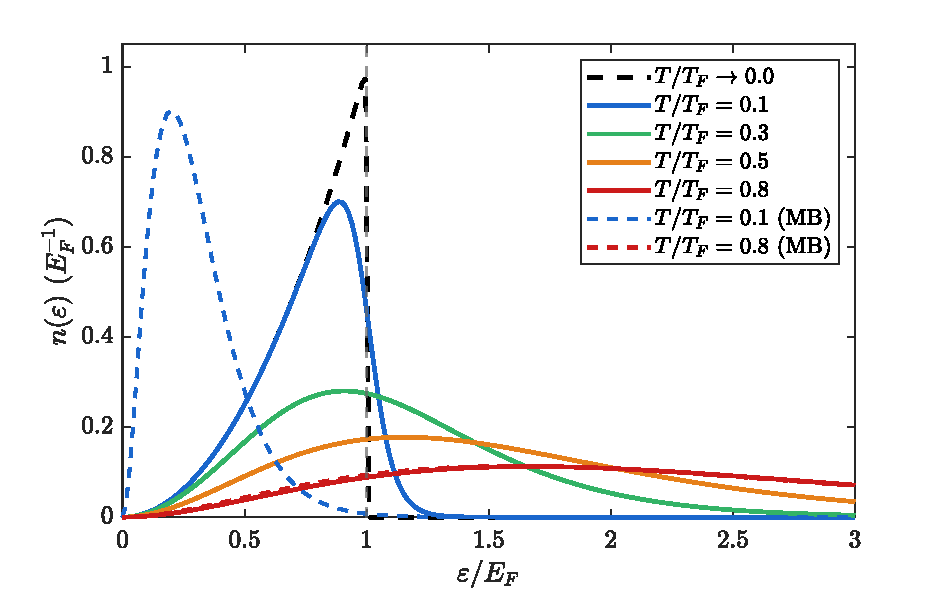
\includegraphics[trim=0cm 0 0cm 0, clip, width=0.9\columnwidth]{gfx/Cpt2_fig/FermiDirac.pdf}
	\caption{Energy distribution $n(\varepsilon)=g(\varepsilon)f_{\mathrm{FD}}(\varepsilon)$ of an ideal Fermi gas in a three-dimensional harmonic trap for different values of $T/T_F$. The black dashed curve indicates the zero-temperature limit, where all states below $E_F$ are occupied. The dashed Maxwell--Boltzmann curves illustrate the corresponding classical distributions. All curves are shown in arbitrary units. \label{fig:FDdistro}}
\end{figure}
In Fig.~\ref{fig:FDdistro}, we summarize the behavior of an ideal Fermi gas close to degeneracy, by plotting the energy distribution $n(\varepsilon)=g(\varepsilon)f_{\mathrm{FD}}(\varepsilon)$ for different values of $T/T_F$, with $g(\varepsilon)=\varepsilon^2/(\hbar\bar\omega)^3$ is the three dimensional density of states. We compare the energy distribution of a Fermi gas at different temperatures with the energy distribution of a classical gas, which adheres to the Maxwell-Boltzmann distribution. For very low temperatures ($T/T_F\to0$), the Pauli principle leads to a filling of the Fermi sea, resulting in a large discrepancy between the two distributions. At higher temperatures, instead, the the Fermi--Dirac distribution is washed out by thermal fluctuations and the Maxwell-Boltzmann distribution is recovered.
%The red dashed line indicates the case of a thermal gas according to the Maxwell-Boltzmann distribution, while the black dashed line indicates the case of $T/T_F\to0$. The solid lines show how, lowering the temperature, the low energy states get filled up and the Fermi-Dirac distribution deviates from the expected behavior of a thermal gas. The gray dashed line shows the expected distribution for a thermal gas with the same temperature of the solid blue line, $T/T_F=0.1$.  

In ultracold-gas experiments, the degree of degeneracy of a Fermi gas is commonly quantified by the ratio $T/T_F$. If the temperature of the gas is below the Fermi temperature, $T/T_F<1$, the gas is said to be degenerate. This is analogous to the bosonic case, where degeneracy is signaled by $T<T_c$; however, unlike bosons, an ideal Fermi gas does not undergo a phase transition. Instead, the crossover to degeneracy is smooth and corresponds to the progressive filling of the Fermi sea.


Experimentally, the onset of Fermi degeneracy manifests itself as a deviation of the atomic cloud profile, observed after \ac{TOF}, from the Gaussian profile expected for a classical thermal gas. This deviation serves as a direct measure of degeneracy, and in practice it is extracted from fit of two-dimensional column density profiles obtained from absorption imaging with a polylogarithmic function \cite{Ketterle2008mpa}
\begin{equation}
	n(x,y) = -A\,\frac{\mathrm{Li}_2\left(-z \exp\left(-\frac{x^2}{2\sigma_x^2} - \frac{y^2}{2\sigma_y^2}\right)\right)}{\mathrm{Li}_2\left(-z\right)},
	\label{eq:PolyLog}
\end{equation} 
where $ \mathrm{Li}_2$ is the polylogarithm of order $2$, $A$ is an amplitude, $z=e^{\mu/k_BT}$ is the fugacity, and $\sigma_{x,y}$ are the thermal widths. The fugacity $z$ encodes the degeneracy: for $z\ll 1$ the distribution reduces to a Gaussian (classical limit), while for $z\gg1$ the distribution approaches the zero-temperature Thomas-Fermi profile. The ratio  $T/T_F$ is then extracted from the fitted fugacity via:
\begin{equation}
	\frac{T}{T_F} = \left[-6\,\mathrm{Li}_3(-z)\right]^{-1/3},
\end{equation}
where $ \mathrm{Li}_3$ is the polylogarithm of order $3$, which accounts for the three-dimensional density of states.

It is worth noting here that these definitions and quantities are valid for a non interacting Fermi gas. In such a gas, low-energy $s$-wave collisions  are forbidden by antisymmetry of the many-body wave function, and higher partial waves are suppressed at ultracold temperatures. This suppression of elastic collisions is one of the reasons why ultracold Fermi gases are commonly studied in mixtures, where distinguishable particles can interact through the $s$-wave channel. The remainder of this chapter introduces the scattering concepts needed to describe these interactions and their magnetic-field control through Feshbach resonances.


% In the case of spin mixtures the different components share the same mass and optical properties, i.e.~the same trapping frequencies. In the case of

%mention deformation of Fermi surface from dipolar interaction observed in Er


\section{Basics of scattering theory}
\label{sec:ScatteringTheo}

At the low densities and temperatures of ultracold gases, interactions between distinguishable particles can be described to a very good approximation in terms of two-body scattering. In this section, we introduce the basic scattering quantities needed to characterize such interactions.

We consider two particles interacting through a potential $V(r)$ that depends only on their relative distance. Far from the interaction region, the scattering wave function can be written as the sum of an incoming plane wave and an outgoing spherical wave,
\begin{equation}
	\psi_k(r)\sim e^{ikz}+f(k,\theta)\frac{e^{ikr}}{r},
	\label{eq:wavefunScatt}
\end{equation}
where $\mathbf{k}$ is the relative wave vector and $f(k,\theta)$ is the scattering amplitude. The differential cross section is obtained directly from the scattering amplitude as
\begin{equation}
\frac{d\sigma}{d\Omega}=|f(k,\theta)|^2.
\label{eq:diffCrossSec}
\end{equation}
	
For a central potential, the scattering problem can be decomposed into partial waves of angular momentum quantum number $l$. Each partial wave experiences an effective radial potential	
\begin{equation}
	V_{\mathrm{eff}}(r)=\frac{\hbar^2l(l+1)}{2m_rr^2}+V(r)
	\label{eq:effPot}
\end{equation}
where $m_r$ is the reduced mass of the two body problem, and the first term of this relation is the centrifugal barrier. The effect of the interaction in each partial wave is encoded in a phase shift $\delta_l(k)$. The contribution of each partial wave to the total cross section is then
\begin{equation}
	\sigma_l(k)=\frac{4\pi}{k^2}(2l+1)\sin^2(\delta_l(k)).
	\label{eq:crossSecpartialWave}
\end{equation}

For low collision energies, which is usually the case for ultracold gases, higher partial waves, with $l>0$, are strongly suppressed, and only the $s$-wave channel, with $l=0$, survives. In the specific case of our experiment, this is not valid for Dy. For strongly magnetic atoms, the long-range and anisotropic dipole-dipole interaction enables higher-partial-wave scattering even at very low temperatures. Nonetheless, the interspecies interaction in the Dy-K mixture, relevant to most of the results presented in this thesis, is still well described within the contact interaction framework.

For the $s$-wave channel, the low-energy scattering properties are summarized by the scattering length $a$, defined through the zero-energy limit of the phase shift,
\begin{equation}
	a=\lim_{k\to0}\frac{\tan(\delta_0(k))}{k}.
	\label{eq:ScatteringLength}
\end{equation}
The corresponding $s$-wave scattering amplitude is
\begin{equation}
	f(k)=\frac{1}{-\frac{1}{a}+\frac{1}{2}r_{\textrm{eff}}k^2-ik},
	\label{eq:ScatteringAmplswave}
\end{equation}
where $r_{\mathrm{eff}}$ is the effective range. Integrating the differential cross section over solid angle, we can obtain the total cross section for the $s$-wave channel
\begin{equation}
	\sigma(k)=\frac{4\pi}{\left(\frac{1}{a}-\frac{1}{2}r_{\textrm{eff}}k^2\right)^2+k^2}.
\end{equation}
In the limit where effective-range corrections can be neglected,
\begin{equation}
	\sigma(k)=\frac{4\pi a^2}{1+k^2a^2}.
	\label{eq:TotalCrossSection}
\end{equation}
In the limit of small scattering length, $ka\ll1$, this becomes $\sigma=4\pi a^2$. For resonant interactions, $|a|\to\infty$, the cross section saturates at the unitarity limit,
\begin{equation}
	\sigma(k)=	\frac{4\pi}{k^2}.
	\label{eq:UniversaCrossSec}
\end{equation}
\albi{put forward reference to the chapter on Hydrodynamics}

The scattering length therefore determines the strength of low-energy interactions in an ultracold gas. In a many-body Fermi system, the relevant dimensionless interaction parameter is $k_Fa$, or equivalently $1/(k_Fa)$. The ability to tune $a$ makes it possible to move from weakly attractive interactions, through the strongly interacting unitary regime, to the molecular side of the resonance, where weakly bound dimers exist. Magnetic Feshbach resonances, introduced in the next section, provide precisely this tunability. \albi{rewrite this}

\section{Feshbach resonances in ultracold gases}
\label{sec:FeshbachResIntro}


Magnetically tunable Feshbach resonances are one of the central tools of ultracold-atom experiments. They allow the interaction strength between two atoms to be controlled by changing an external magnetic field. Here we summarize the key quantities and results relevant to the contents of this thesis, for a detailed overview of Feshbach resonances in ultracold gases, we refer to Ref.~\cite{Chin2010fri}, which is the standard reference for the topic. 

\begin{figure}[thb]
	\centering
	\includegraphics[trim=0cm 0 0cm 0, clip, width=0.9\columnwidth]{gfx/Cpt2_fig/FeshbachRes.pdf}
	\caption{Two channel model for a Feshbach resonance. Scattering is resonantly enhanced when the collision energy of two atoms in the open channel is coupled to a bound state of the closed channel potential $V_c$, in red.  \label{fig:FeshbachResonance}}
\end{figure}
The two-channel model for a Feshbach resonance is illustrated in Fig.~\ref{fig:FeshbachResonance}.The tunability of the scattering length originates, at the two-body level, from the coupling between the open scattering channel, and a molecular bound state $E_c$ supported by a closed channel potential. The two channels generally have different magnetic moments, so that the energy of the bound state relative to the scattering threshold can be tuned by varying an external magnetic field. When this energy is tuned close to the scattering threshold, the scattering length is resonantly enhanced and can be tuned over a wide range. On the repulsive side of the resonance, the two-atom system supports a weakly bound molecular state, commonly referred to as a Feshbach molecule.

\begin{figure}[thb]
	\centering
	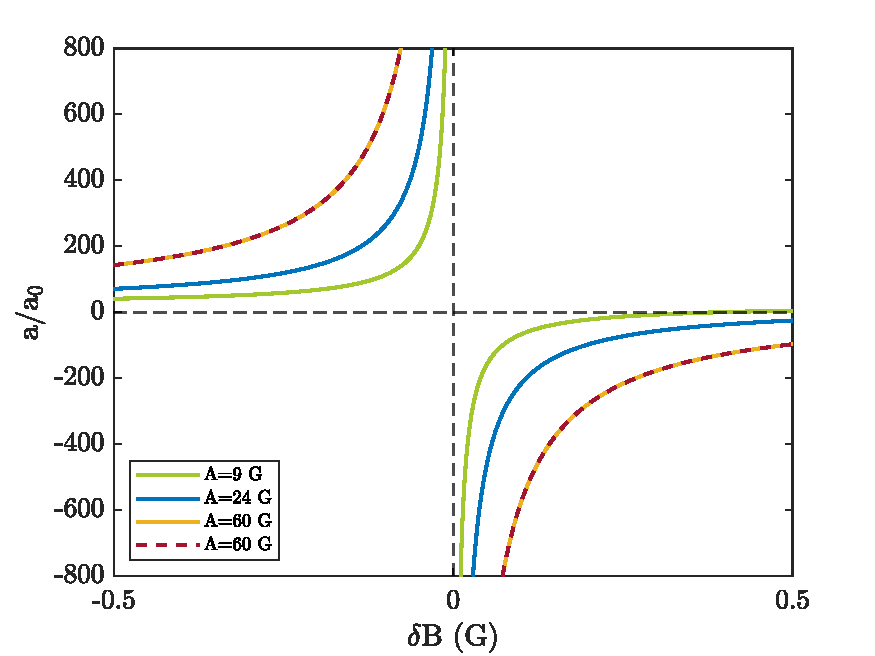
\includegraphics[trim=0cm 0 0cm 0, clip, width=0.9\columnwidth]{gfx/Cpt2_fig/Feshbachres_varyingA.pdf}
	\caption{Scattering length near a Feshbach resonance for different values of the pole strength $A$. The yellow and red curves overlap because they have the same value of $A$. The blue curve shows the scattering length for the resonance near \SI{7}{G}, using the parameters characterized in this thesis. \label{fig:ScatteringLengthDiffAINtro}}
\end{figure}
Near a well-isolated Feshbach resonance, the scattering length as a function of magnetic field $B$, can be expressed in terms of few parameters \cite{Moerdijk1995riu}
\begin{equation}
	a(B)=a_{bg}-\frac{A}{B-B_0},
	\label{eq:scatteringLength}
\end{equation}
where $B_0$ is the resonance pole, $a_{bg}$ is the background scattering length far from the resonance, and $A$ is the strength parameter, related to the resonance width $\Delta$ by $A=\Delta a_{bg}/a_0$. In Fig.~\ref{fig:ScatteringLengthDiffAINtro}, we show examples of resonances with different strength parameters for a fixed $B_0$ and $a_{bg}$.

In the limit of large scattering length $a$, the binding energy of the Feshbach molecular state can be expressed as
\begin{equation}
	E_b=\frac{\hbar^2}{2m_ra^2}.
	\label{eq:BindingEnergyUniv_Intro}
\end{equation}
In this region, the bound state acquires a universal character, and can be described in terms of the scattering length $a$ alone. This universal expression holds particularly well near broad, open-channel dominated resonances where the effective range $r_{\mathrm{eff}}$ is small and its corrections to Eq.~\eqref{eq:BindingEnergyUniv_Intro} remain negligible over a wide range of magnetic fields. One of the Feshbach resonances between different spin states of $^6$Li is a prominent example of such a case. The exceptionally large width of this resonance has enabled a remarkable variety of experiments and has been defined anecdotally multiple times as a ``gift of Nature'' \cite{Jochim2003bec, Varenna2006book}. \albi{cite more}

In the case of Dy-K, Nature has been a bit less generous, and most of the interspecies resonances found so far lie within the classification of narrow Feshbach resonance. The next section therefore serves as a brief compendium on narrow Feshbach resonances.



\section{Narrow Feshbach resonances}
\label{sec:NarrowFR}

Narrow,  or closed-channel dominated resonances occur when the coupling between the two channels is weak and the underlying bound state retains a predominantly closed-channel character over a wide field range. In this case, the three parameters  ($A$, $a_{bg}$, and $B_0$) introduced previously are no longer sufficient to fully characterize the scattering properties near the resonance, and an additional parameter is required. In $2004$, D.~Petrov introduced the characteristic length scale $R^*$, related to the effective range by $R^*=-r_{\mathrm{eff}}/2$, defined as \cite{Petrov2004tbp}
\begin{equation}\label{eq:Rstar}
	R^*=\frac{\hbar^2}{2m_ra_0\delta\mu A},
\end{equation}
where $\delta\mu=\mu_{\mathrm{open}}-\mu_{\mathrm{closed}}$ is the differential magnetic moment between the closed and open channels.

The binding energy of the molecular state for a narrow resonance can then be  expressed as
\begin{equation}\label{eq:BindingEnergy_Intro}
	E_b=\frac{\hbar^2}{8(R^*)^2m_r}\left(\sqrt{1-\frac{4R^*(B-B_0)}{a_0 A}}-1 \right)^2.
\end{equation}
In the limit of $|a|\gg R^*$, the scattering properties of the two-body system recover their universal character, and the binding energy reduces to the universal expression of Eq.~\eqref{eq:BindingEnergyUniv_Intro}.

\begin{figure}[thb]
	\centering
	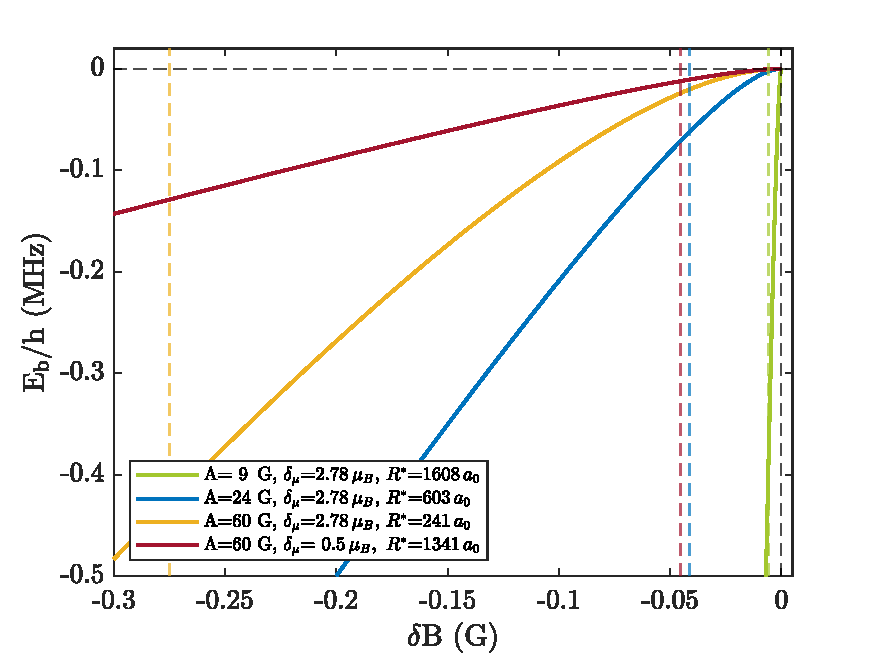
\includegraphics[trim=0cm 0 0cm 0, clip, width=0.9\columnwidth]{gfx/Cpt2_fig/Feshbachres_BindingEnergies.pdf}	
	\caption{Binding energy $E_b/\hbar$ as a function of magnetic field detuning $\delta B=B-B_0$ for four narrow Feshbach resonances with different strength parameters $A$ and differential magnetic moments $\delta\mu$. The vertical dashed lines indicate the characteristic detuning at which $|a|=R^*$ for each resonance. The dashed black horizontal line marks the free-atom threshold $E_b=0$.\label{fig:narrowFRBinding}}\albi{change the order of the lines in the legend}
\end{figure}
The parameter $R^*$ determines the range of detunings over which the resonance behaves universally. The apparent width of a narrow resonance is therefore governed by the accessibility of the regime $|a|\gg R^*$. This behavior is illustrated in Fig.~\ref{fig:narrowFRBinding}. The green, blue, and yellow curves correspond to increasing values of $A$ at fixed $\delta\mu$. The vertical dashed lines indicates the magnetic fields for which the condition $|a|=R^*$ is satisfied. As $A$ increases, $R^*$ decreases and the resonance becomes progressively less closed-channel-dominated. Consequently, the universal binding-energy relation remains valid over a wider interval of magnetic-field detunings. For the smallest value, $A=\SI{9}{G}$, the condition $|a|=R^*$ is reached only very close to the resonance pole, while for $A=\SI{60}{G}$ it occurs at detunings of order a few hundred \unit{mG}.

The comparison between the yellow and red curves highlights that the scattering length alone does not fully determine the near-threshold molecular spectrum of a narrow resonance. These two curves have the same value of $A$ and therefore the same scattering length $a(B)$, as shown in Fig.~\ref{fig:ScatteringLengthDiffAINtro}. However, they differ in $\delta\mu$, and therefore in $R^*$. The smaller differential magnetic moment of the red curve leads to a larger $R^*$ and to a more closed-channel dominated molecular state. As a result, the binding energy deviates more strongly from the universal expression, even though the corresponding scattering-length curve is identical.

The molecular bound state underlying a resonance can be directly populated forming weakly bound molecules, as we will see in more detail in Part~\hyperref[pt:MakingProbing]{III}. Therefore, it is useful to the differential magnetic moment of the molecular state, an additional quantity of direct experimental relevance, which is obtained by differentiating the binding energy with respect to the magnetic field
\begin{equation}\label{eq:MagneticMoment_Intro}
	\delta\mu_{\mathrm{mol}}=\frac{\partial E_b}{\partial B}=\delta\mu\left(1-\frac{1}{\sqrt{1-\frac{4R^*(B-B_0)}{a_0 A}}}\right).
\end{equation}
Here $E_b$ is defined as the molecular energy relative to the free-atom threshold and is therefore negative for a bound state. Far from the resonance pole, $\delta\mu_{\mathrm{mol}}$ approaches $\delta\mu$, corresponding to the bare closed-channel molecular state. Close to the pole, instead, $\delta\mu_{\mathrm{mol}}\to0$, reflecting the increasing open-channel character of the weakly bound molecule. We can then introduce the closed-channel fraction
\begin{equation}\label{eq:ClosedChannelFraction_Intro}
	Z(B)=\delta\mu_{\mathrm{mol}}(B)/ \delta\mu,
\end{equation}
which quantify the admixture between the bare closed-channel molecular state and the open-channel scattering state.

\begin{figure}[thb]
	\centering
	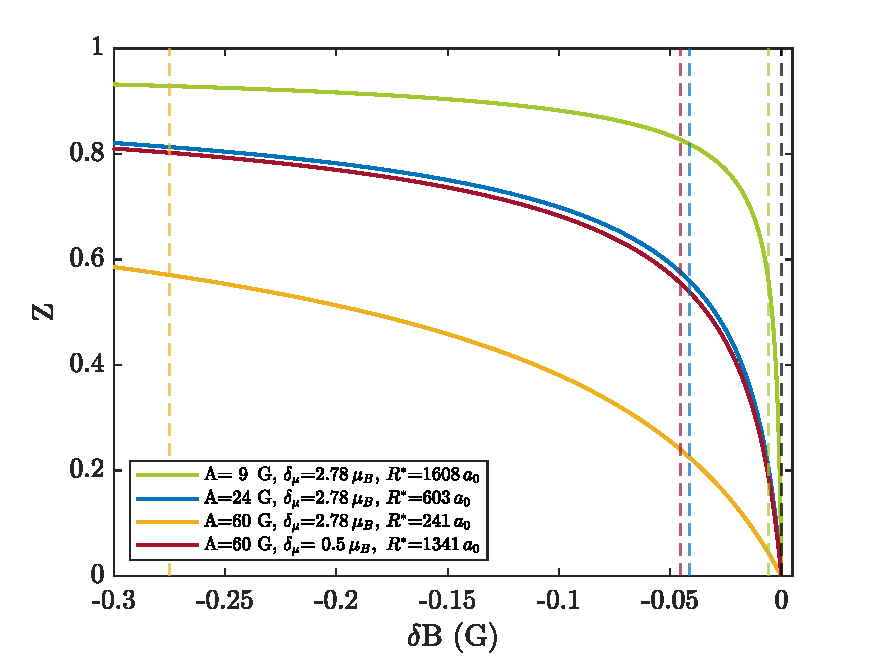
\includegraphics[trim=0cm 0 0cm 0, clip, width=0.95\columnwidth]{gfx/Cpt2_fig/Feshbachres_Z.pdf}
	\caption{Closed-channel fraction $Z(B)$ as a function of magnetic field detuning  $\delta B=B-B_0$ 	for the same four resonances shown in Fig.~\ref{fig:narrowFRBinding}. The vertical dashed lines indicate the characteristic detunings at which $|a|=R^*$, marking the crossover between the universal open-channel-dominated regime close to the pole and the closed-channel-dominated behavior at larger detuning \label{fig:narrowFRZ}}
\end{figure}
In Fig.~\ref{fig:narrowFRZ}, we compare the behavior of $Z(B)$ for the different narrow-resonance examples introduced above. Close to the resonance pole, $B\to B_0$, the closed-channel fraction vanishes, $Z\to0$, reflecting the fact that the weakly bound molecule becomes increasingly open-channel dominated and acquires universal character. Far from the pole, instead, $Z$ approaches unity and the molecule recovers the character of the bare closed-channel bound state. The vertical dashed lines indicate the characteristic detunings at which $|a|=R^*$, as in Fig.~\ref{fig:narrowFRBinding}. They mark the crossover scale between the universal, open-channel-dominated region close to the pole and the closed-channel-dominated behavior at larger detuning. Increasing either the strength parameter $A$ or the differential magnetic moment $\delta\mu$ reduces $R^*$ and broadens the field range over which $Z$ remains small. Conversely, small values of $A$ or $\delta\mu$ lead to large $R^*$ and to molecules that retain a large closed-channel fraction except extremely close to resonance. 






%In the green resonance case, the strength parameter is the smallest considered here, $A=\SI{9}{G}$, see also the green line in Fig.~\ref{fig:ScatteringLengthDiffAINtro}, and thus the resonance is closed-channel dominated and the universal behavior can be recovered only for very small detunings from the resonance pole. Keeping $\delta\mu$ fixed, we can considered other two cases with larger strength parameters, the blue and yellow lines, with $A=\SI{24}{G}$ and $A=\SI{60}{G}$, respectively. In this case the resonances get progressively more open-channel dominated, and the universal regime can be recover for larger values of $\delta B$, in particular for the yellow curve where the universal regime can be recovered for detunings of hundreds of \unit{mG}. 


%\begin{equation}\label{eq:BindingEnergyBstar_Intro}
%	E_b=\delta_\mu \delta B^*\left(\sqrt{1-\frac{\delta B}{\delta B^*}}-1\right)^2
%\end{equation}


%\begin{equation}
%	\delta B^* =\frac{m_r\delta_\mu A^2 a_0^2}{2\hbar^2}
%\end{equation}


%\begin{equation}
%	\delta\mu_{\mathrm{mol}}=\partial E_{\mathrm{mol}}/\partial B=\delta\mu\left(1-\frac{1}{\sqrt{1-\frac{\delta B}{\delta B^*}}}\right).
%\end{equation}


%\[|\delta B_{R^*}|=\frac{2m_r\delta\mu(a_0A)^2}{\hbar^2}.\]




%It is then clear that a narrow resonance can appear ``broader'' in character by how feasible is to access the limit $|a|\gg R^*$. A closer inspection of Eq.~\eqref{eq:Rstar}, shows that the strength parameter $A$ and the differential magnetic moment $\delta\mu$ combine to determine the values of $R^*$ and the ease of accessibility of the universal range. To explore this, in Fig.~\ref{fig:narrowFRBinding} we compare the behavior of bound states of different narrow Feshbach resonances, using the values of $A$ presented in Fig.~\ref{fig:ScatteringLengthDiffAINtro}, combined with two different values of $\delta_\mu$. The vertical dashed lines in Fig.~\ref{fig:narrowFRBinding} show the $\delta B$ field values for which the condition $|a|=R^*$ is satisfied.



%However, as said before, the strength parameter is not enough to characterize the behavior of the resonances. We consider a fourth example, which uses also $A=\SI{60}{G}$, but a smaller $\delta\mu$, showed in red in the figures. While in Fig.~\ref{fig:ScatteringLengthDiffAINtro}, the yellow and the red lines perfectly overlap, in Fig.~\ref{fig:narrowFRBinding}, the molecular states underlying the resonances differ between each other. Moreover, for the red curve, the condition $|a|=R^*$ is satisfied only at much smaller detunings compared to the yellow one, an it is almost the same as the one of the blue resonance. 

